%https://www.khronos.org/registry/OpenGL/specs/gl/glspec46.core.pdf 

\section{OpenGL}
\todo{talk a bit about openGL, implementors and programmers perspective, Look at section 1.2 of spec}
\todo{talk about general dataflow model of OpenGL and show bits that are relevant to my project, Look at Chapter 3 of spec}
\begin{figure}
    \centering
    \includegraphics{}
    \caption{Caption}
    \label{fig:my_label}
\end{figure}
Relevant parts are the structure of the inputs and outputs of the rasterizer stage which come from the geometry processing stage and go to the fragment shader stage both of which are programmable.
\todo{insert dataflow model block diagram, found at page 35 of the openGL 4.6 Spec. }
\subsection{Vertex Representation}
OpenGL actually only passes triangle strips to the ratseriser from the geometry processing stage, as well as lines and points. The following section described the various triangle representations
\subsection{Triangle Representation}
\subsubsection{Individual Triangles}
Separate triangles are specified with mode TRIANGLES. In this case, the $3i + 1$, $3i + 2$, and $3i + 3$ vertices (in that order) determine a triangle for each $i = 0, 1, ... , n - 1$, where there are $3n + k$ vertices drawn. $k$ is either 0, 1, or 2; if \textit{k} is not zero, the final $k$ vertices are ignored. For each triangle, vertex \textit{A} is vertex $3i$ and vertex \textit{B} is vertex $3i + 1$. Otherwise, separate triangles are the same as a triangle strip.
\subsubsection{Triangle Strips}
A triangle strip is a series of triangles connected along shared edges, and is specified with mode TRIANGLE\_STRIP. In this case, the first three vertices define the first triangle (and their order is significant). Each subsequent vertex defines a new triangle using that point along with two vertices from the previous triangle. If fewer than three vertices are specified, no primitive is produced, \Cref{fig:TriangleRepresentationOpenGL}. The required state consists of a flag indicating if the first triangle has been completed, two stored processed vertices (called vertex A and vertex B), and a one bit pointer indicating which stored vertex will be replaced with the next vertex. When a series of vertices are transferred to the GL, the pointer is initialized to point to vertex A. Each successive vertex toggles the pointer. Therefore, the first vertex is stored as vertex A, the second stored as vertex B, the third stored as vertex A, and so on. Any vertex after the second one sent forms a triangle from vertex A, vertex B, and the current vertex (in that order).
\subsubsection{Triangle Fans}
A triangle fan is specified with mode TRIANGLE\_FAN, and is the same as a triangle strip with one exception: each vertex after the first always replaces vertex B of the two stored vertices.

\begin{figure}[ht]
    \centering
    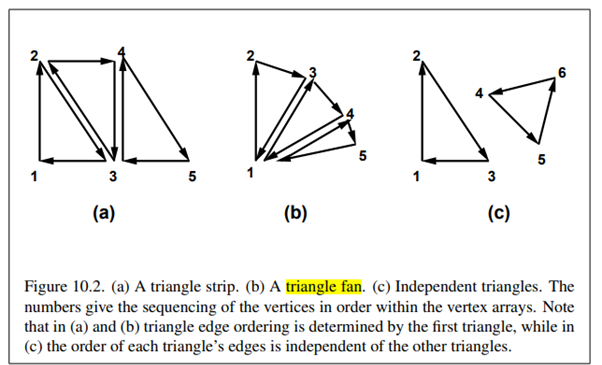
\includegraphics{lit_review/images/TriangleRepresentationOpenGLDiagram.png}
    \caption{Caption}
    \label{fig:TriangleRepresentationOpenGL}
\end{figure}
\todo{What are the advantages and disadvantages of each triangle data structure}
\todo{Is the rasterization of each of these different?}
\todo{Do they provide performance benefits?}

\subsubsection{Winding Order}
In Figure \ref{fig:tetrahedron_description}, the indices for the vertices that describe each face are defined with a \textbf{winding order}. The winding order can be either clockwise or anti clockwise. This means that the vertices that define a triangle are listed in clockwise order when looking at the front side of the triangle. The lowest index always comes first as shown in Figure \ref{fig:triangle_winding_order}.
\begin{figure}[ht]
    \centering
    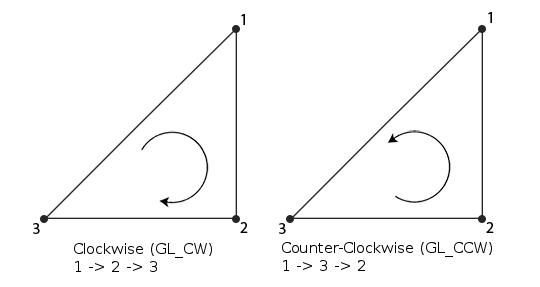
\includegraphics{lit_review/images/triangle_winding_order.png}
    \caption{https://www.khronos.org/opengl/wiki/Face\_Culling}
    \label{fig:triangle_winding_order}
\end{figure}
Figure \ref{fig:tetrahedron_description} shows the description of a tetrahedron composed of triangles with a clockwise winding order.
\begin{figure}[ht]
    \centering
    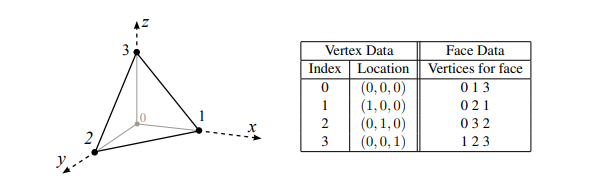
\includegraphics{lit_review/images/tetrahedron_description.png}
    \caption{Provides an example of location and face data used to describe a tetrahedron.(insert reference to GraphicsNotes01.pdf)}
    \label{fig:tetrahedron_description}
\end{figure}

The ordering convention chosen doesn't matter as long as its consistent between all triangles in the same scene. The reason this convention is needed is primarily for triangle culling where to accelerate the rasterization process, any triangles that are facing away from the camera (and so assumed to be on the back side of objects) are not rendered. This reduces the number of triangles rendered and so speeds up the rendering process. [https://www.khronos.org/opengl/wiki/Face\_Culling]

\subsubsection{Polygons}
A polygon is defined by the specification as: A polygon results from a triangle arising from a triangle strip, triangle fan, or series of separate triangles.
I will therefore assume that the rasterization block will be passed a list of polygons (individual triangles). This list will be produced by the primitive assembly stage implemented in software which will parse a set of triangles, triangle strips or triangle fans into a list of polygons.

\subsection{Fragment Representation}
OpenGL spec section 15.2.2 Shader Inputs

\todo{describe what a fragment actually is and how it is stored}
\subsection{Rasterization in OpenGL}\label{sec:rasterOpenGL}

The rasterization stage is the one I will be focusing on for the MVP of the project. It contains these stages as described by the OpenGL spec:

\begin{itemize}
    \item Face Culling
    \item Project Triangles to screen space
    \item Checking if a pixel lies in a projected triangle
    \item Triangle Clipping in screen space
    \subitem Triangles may be turned into quads as a result of this
    \item Interpolation of vertex attributes including depth
\end{itemize}

\subsubsection{Interpretation of polygons (face, mode)}
\begin{table}[ht]
    \begin{tabular}{|l|l|l|}
    \hline
    Face             & Mode  & Note                                                 \\ \hline
    FRONT\_AND\_BACK & POINT & Vertices are rasterized as points                    \\ \hline
    FRONT\_AND\_BACK & LINE  & Polygon edges are rasterized as line segments        \\ \hline
    FRONT\_AND\_BACK & FILL  & rasterize polygon as described in following sections \\ \hline
    \end{tabular}
    \caption{Caption}
    \label{table:OpenGLrasterizerModes}
\end{table}
For the purposes of the \textit{rasterizeTriangles} instruction Mode is always set to FILL, \Cref{table:OpenGLrasterizerModes}. However, I will leave in the parameter to allow building a line and point rasterizer accelerators as an extension to the project.
\subsubsection{Determine if the triangle is front or back facing (winding order) - always done}
This is computed based on the (unclipped/clipped) polygon’s area computed in window coordinates. 
It is also computed based on a customisable winding order.

\subsubsection{Face culling (mode, enable)}
Face culling is an important optmisation in rendering. Those triangles that are facing away from the camera and so definitely cannot be seen are not rasterized or "culled". This significantly reduces the number of triangles that need to be rendered by the GPU and saves huge amounts of time when rendering a scene.

In openGL, back facing triangles are rasterized by default but there are pipeline parameters \textbf{mode} and \textbf{enable} which allow the programmer to specify which tringles should be culled. The effects of various parameter setting are show in \Cref{table:faceCullingModes}.
\begin{table}[ht]
    \begin{tabular}{|l|l|l|}
    \hline
    Enable & Mode             & Note                                                \\ \hline
    1      & BACK             & front facing rasterized, back facing not rasterized \\ \hline
    1      & FRONT            & front facing not rasterized, back facing rasterized \\ \hline
    1      & FRONT\_AND\_BACK & nothing rasterized                                  \\ \hline
    0      & anything         & everything rasterized                               \\ \hline
    \end{tabular}
    \caption{Caption}
    \label{table:faceCullingModes}
\end{table}

\subsubsection{Orthographic Projection}
Just take the x and y coordinates of the vertices of the triangle to map the to screen space. This is part of the rasterization stage. It is likely that other projections will be done in the vertex processing stage with shaders.

Doing this projection means that you don't lock the user into a specific type of projection. Gives more flexibility to system.

\subsubsection{Point Sampling}
This step determines which fragments are produced by rasterization of a polygon. This involves traversing the pixels in the bounding box of the polygon and checking if they are inside the polygon or not using the edge equations, \Cref{eqn:triangleEdgeFunction01}, \Cref{eqn:triangleEdgeFunction12}, \Cref{eqn:triangleEdgeFunction20}.

When evaluating the edge equations for a given pixel, the point $p$ used is the centre of the pixel being evaluated.

\begin{itemize}
    \item If a fragment center lies inside the projected triangle it is rasterized.
    \item If a fragment center lies exactly on an edge
    \subitem If two polygons lie on either side of a common edge (with identical endpoints) on which a fragment center lies, then exactly one of the polygons results in the production of the fragment during rasterization.
    \subsubitem \todo{I need to define which triangle is used}
\end{itemize}

\subsubsection{Interpolation of arbitrary vertex attributes and z (noperspecitve, flat, provokeMode)}

We define a set of barycentric coordinates for our triangle: \textit{a,b,c} defined in the range $[0:1]$ such that $a + b + c = 1$.
These uniquely specify a point p in the triangle or on the triangle's boundary by fulfilling \Cref{eqn:pInTermsOfABC}.

\begin{equation}\label{eqn:pInTermsOfABC}
    p = ap_a + bp_b + cp_c
\end{equation}

We can calculate \textit{a,b,c} at a point \textit{p} in the triangle using \Cref{eqn:BaryCentricCoordinate}.
\begin{equation}\label{eqn:BaryCentricCoordinate}
    a = \frac{A(p,p_b,p_c)}{A(p_a,p_b,p_c)}, b = \frac{A(p_a,p,p_c)}{A(p_a,p_b,p_c)}, c = \frac{A(p_a,p_b,p)}{A(p_a,p_b,p_c)}
\end{equation}
Where $p_a, p_b, p_c$ are the vertices of the triangle in screen space and $A(x,y,z)$ is the area of the triangle described by points $x,y,z$.

The data associated with the fragment must be sampled at the centre of the fragment.
For a given attribute $f_n$ associated with a vertex $p_n$, $f_n$ can be calculated using \Cref{eqn:InterpolatedAttr}.

\begin{equation}\label{eqn:InterpolatedAttr}
    f = \frac{\frac{af_a}{w_a}+\frac{bf_b}{w_b}+\frac{cf_c}{w_c}}{\frac{a}{w_a}+\frac{b}{w_b}+\frac{c}{w_c}}
\end{equation}

Where $w_a,w_b,w_c$ are the clip coordinates of $p_a,p_b, p_c$. \todo{what are these clip coordinates? Does the GL spec say what they are?}
\todo{Why is the above equation used??}
\todo{why is depth interpolate in a different way?}
Depth is interpolated in its own way using \Cref{eqn:depthInterpolation}.

\begin{equation}\label{eqn:depthInterpolation}
    z = az_a + bz_b + cz_c
\end{equation}

\begin{table}[ht]
    \begin{tabular}{|l|l|l|}
    \hline
    noperspective & flat & Result                                                                                                      \\ \hline
    0             & 0    & Interpolation using equation with f                                                                         \\ \hline
    1             & 0    & Interpolation of all attributes done with the depth interpolation equation                                  \\ \hline
    0             & 1    & No interpolation done, attribute is assigned to be the same as that of the provoking vertex of the triangle \\ \hline
    1             & 1    & n/a                                                                                                         \\ \hline
    \end{tabular}
    \caption{}
    \label{table:interpolationFlags}
\end{table}

\begin{table}[ht]
    \begin{tabular}{|l|l|l|l|}
    \hline
    ProvokeMode               & Triangle & Triangle Fan & Triangle   Strip \\ \hline
    FIRST\_VERTEX\_CONVENTION & i        & i+1          & i                \\ \hline
    LAST\_VERTEX\_CONVENTION  & 3i       & i+2          & i+2              \\ \hline
    \end{tabular}
    \caption{}
    \label{table:provokeModeSettings}
\end{table}

For calculating the provoking vertex of the \textit{i}th polygon in the scene.
The provoking vertex is used mentioned in table \Cref{table:interpolationFlags}.

\subsubsection{Polygon with greater than 3 edges}

Like those produced by clipping a triangle (makes a quad). These polygons will be turned into a set of triangles without adding vertices before entering the rasterizer. This means we only need to do triangle rasterization.
Or can do generalised interpolation using \Cref{eqn:generalisedInterpolation}

\begin{equation}\label{eqn:generalisedInterpolation}
    f = \sum_{i=1}^{n} a_if_i
\end{equation}

Where f is value of the attribute at vertex i and a is the barycentric coordinate corresponding to vertex i. 
Seems much harder to do in hardware though.

\subsection{Anti-Aliasing}
For each fragment produced a coverage value is calculated using \Cref{eqn:aa-coverage}.

\begin{equation}\label{eqn:aa-coverage}
    coverage = \frac{area \; of pixel \; inside \; polygon}{total \; area \; of \; pixel}
\end{equation}

The above f calculated using interpolation is multiplied by the coverage to produce the actual fragment attribute value f’, \Cref{eqn:interpolatedValueAfterAA}.

\begin{equation}\label{eqn:interpolatedValueAfterAA}
    f' = f * coverage
\end{equation}

This prevents jaggies\cite{jaggiesExplanation} from forming and makes likes seem much smoother to the human eye, this is exeplified by \Cref{fig:AAbeforeAndAfter}.

\begin{figure}[ht]
    \centering
    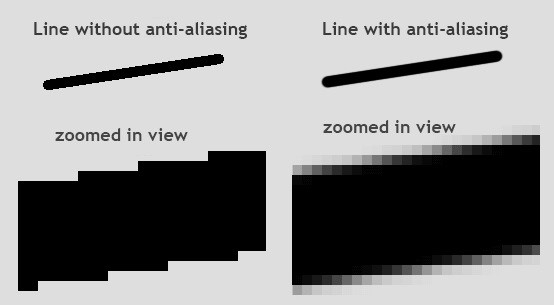
\includegraphics{lit_review/images/BeforeAndAfterAntiAliasing.jpg}
    \caption{Caption\cite{aaDiagram}}
    \label{fig:AAbeforeAndAfter}
\end{figure}